\subsection{Muons}
\label{sec:muonEff}

For the $\Wmn$ cross section determination
the single-muon efficiency combines the efficiencies of all the steps in the muon selection:
triggering on the muon, reconstructing it in the muon and central detectors, and applying the
quality selection and the isolation requirement.
In the procedure followed in this analysis, the reconstruction efficiency in the central tracker is factorized
and  computed independently, while the remaining terms are computed globally, without further
factorizing them into different terms.

An initial preselection of Z events for the \TNP method is performed by selecting
events that contain tracks measured in the central tracker having $\Pt>25$~GeV, $|\eta|<2.1$,
and, when combined with an oppositely charged track, give an
invariant mass in the range $60<m_{\mu^+\mu^-}<120$~GeV. We
further require the presence in the event of a ``tag'' muon, defined as a global muon, that is matched to one of
the preselected tracks, passes the selection described in Section~\ref{sec:muonid}, and corresponds
to an HLT muon. The number of tag muons selected in data is about $22\, 000$. All the other preselected
tracks are considered as probes to evaluate the muon efficiency.
The background present in this sample is subtracted with a fit to the dimuon invariant mass spectrum of the
sum of a Z component and a linear background contribution.
The shape of the Z component is taken from simulation.

The efficiency is studied as a function of the muon $\eta$ and $\Pt$.
A dependence on $\eta$ is observed (Fig.~\ref{rho_eta}, left) because different
regions are covered by different muon detectors.
This behavior is not fully reproduced in
the simulation, as reflected in the corresponding $\rho$ values (Fig.~\ref{rho_eta}, right).
The efficiency also exhibits a dependence on $\Pt$ (Fig.~\ref{rho_pt}, left), but this trend is
similar in data and in simulation, and the correction factors can be taken as approximately constant up to
$\Pt$ = 100~GeV (Fig.~\ref{rho_pt}, right).
 These binned correction factors are applied to the W analysis during signal modeling (Section 8):
W simulated events are weighted with the $\rho$ factor corresponding to the ($\Pt$, $\eta$) bin of the muon.
The slightly difference between the kinematic characteristics of the muons and those from W decays is thus taken into account.

%This variation has been applied in the analysis and ensures that muons, either
%oming from Z or W decays, are treated correctly, without requiring a further correction due to the slight
%ifference in muon kinematic distributions of leptons originating from W or Z bosons.

\begin{figure}
  \begin{center}
  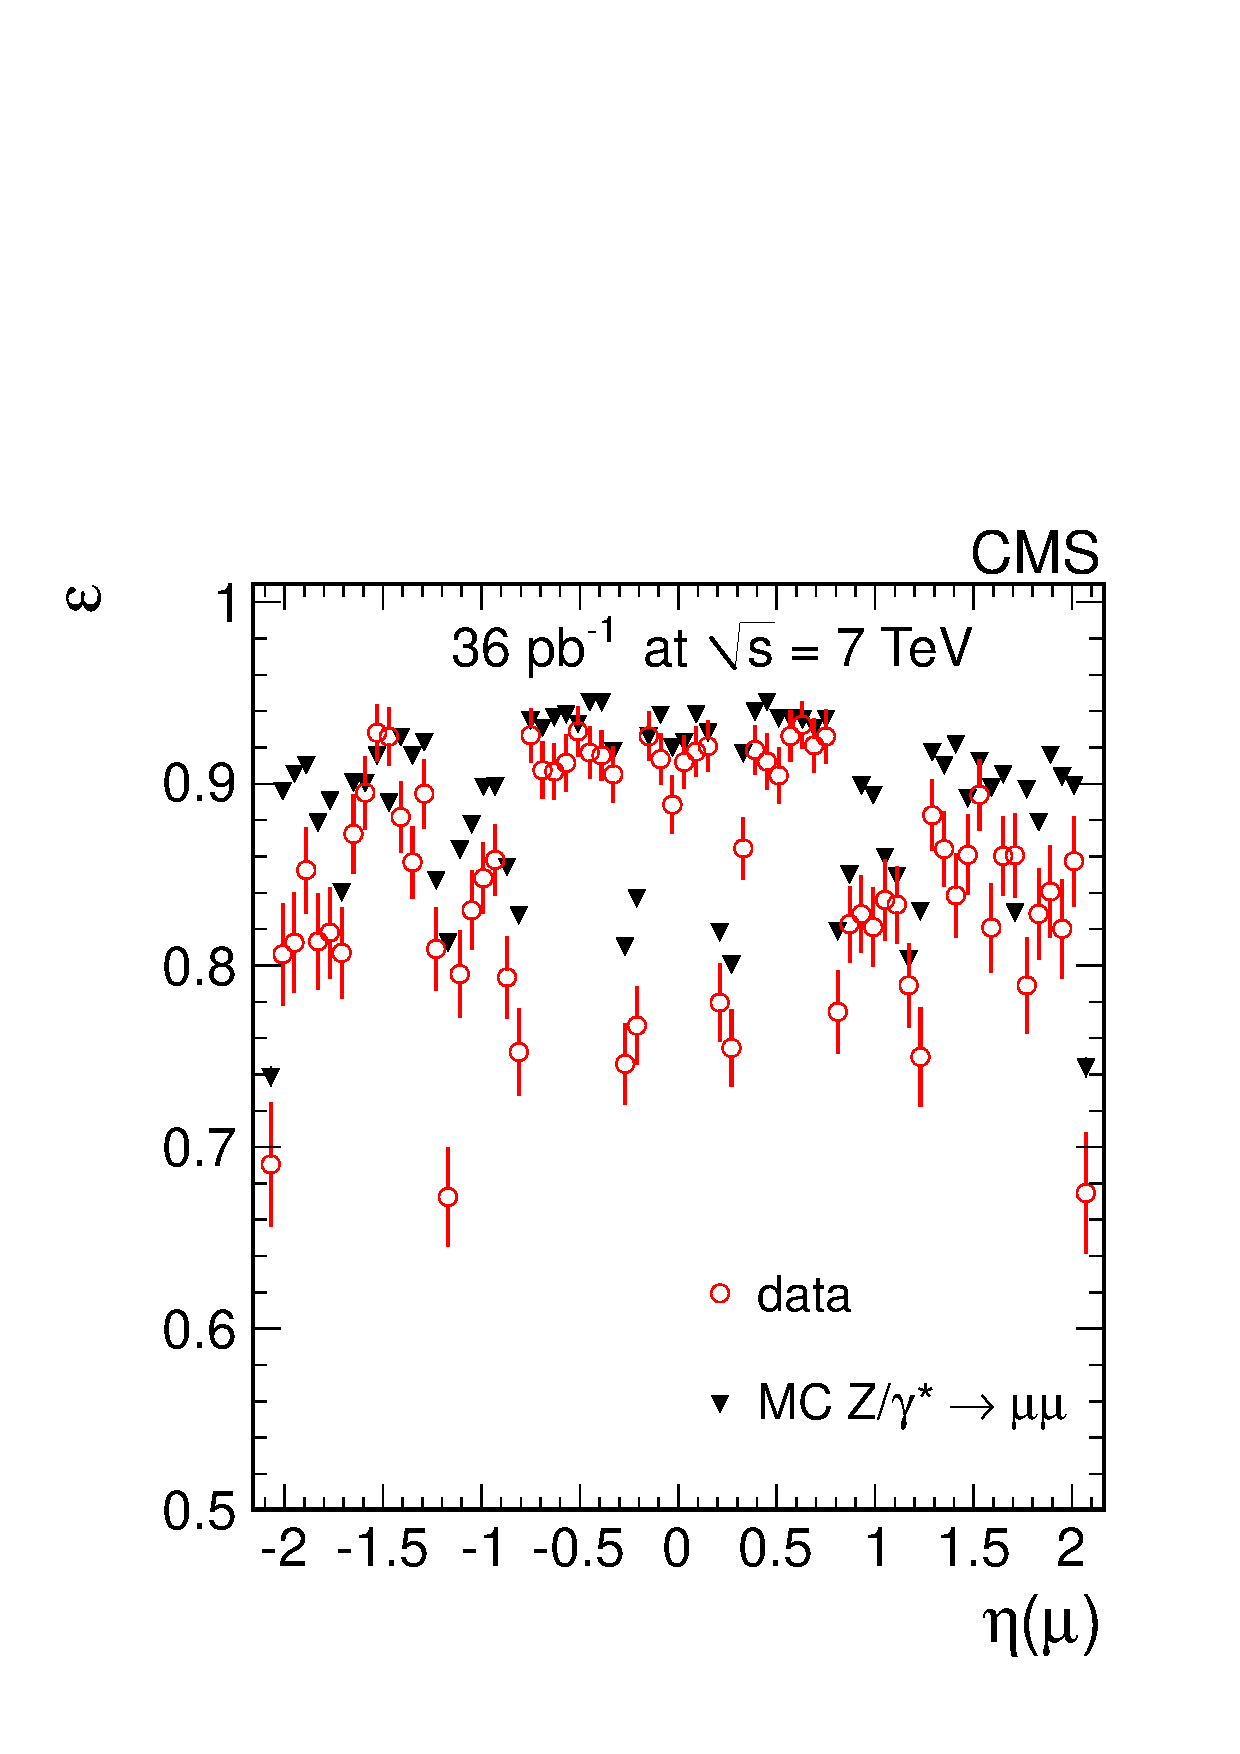
\includegraphics[width=7cm]{figs/efficiency_eta.pdf}%
  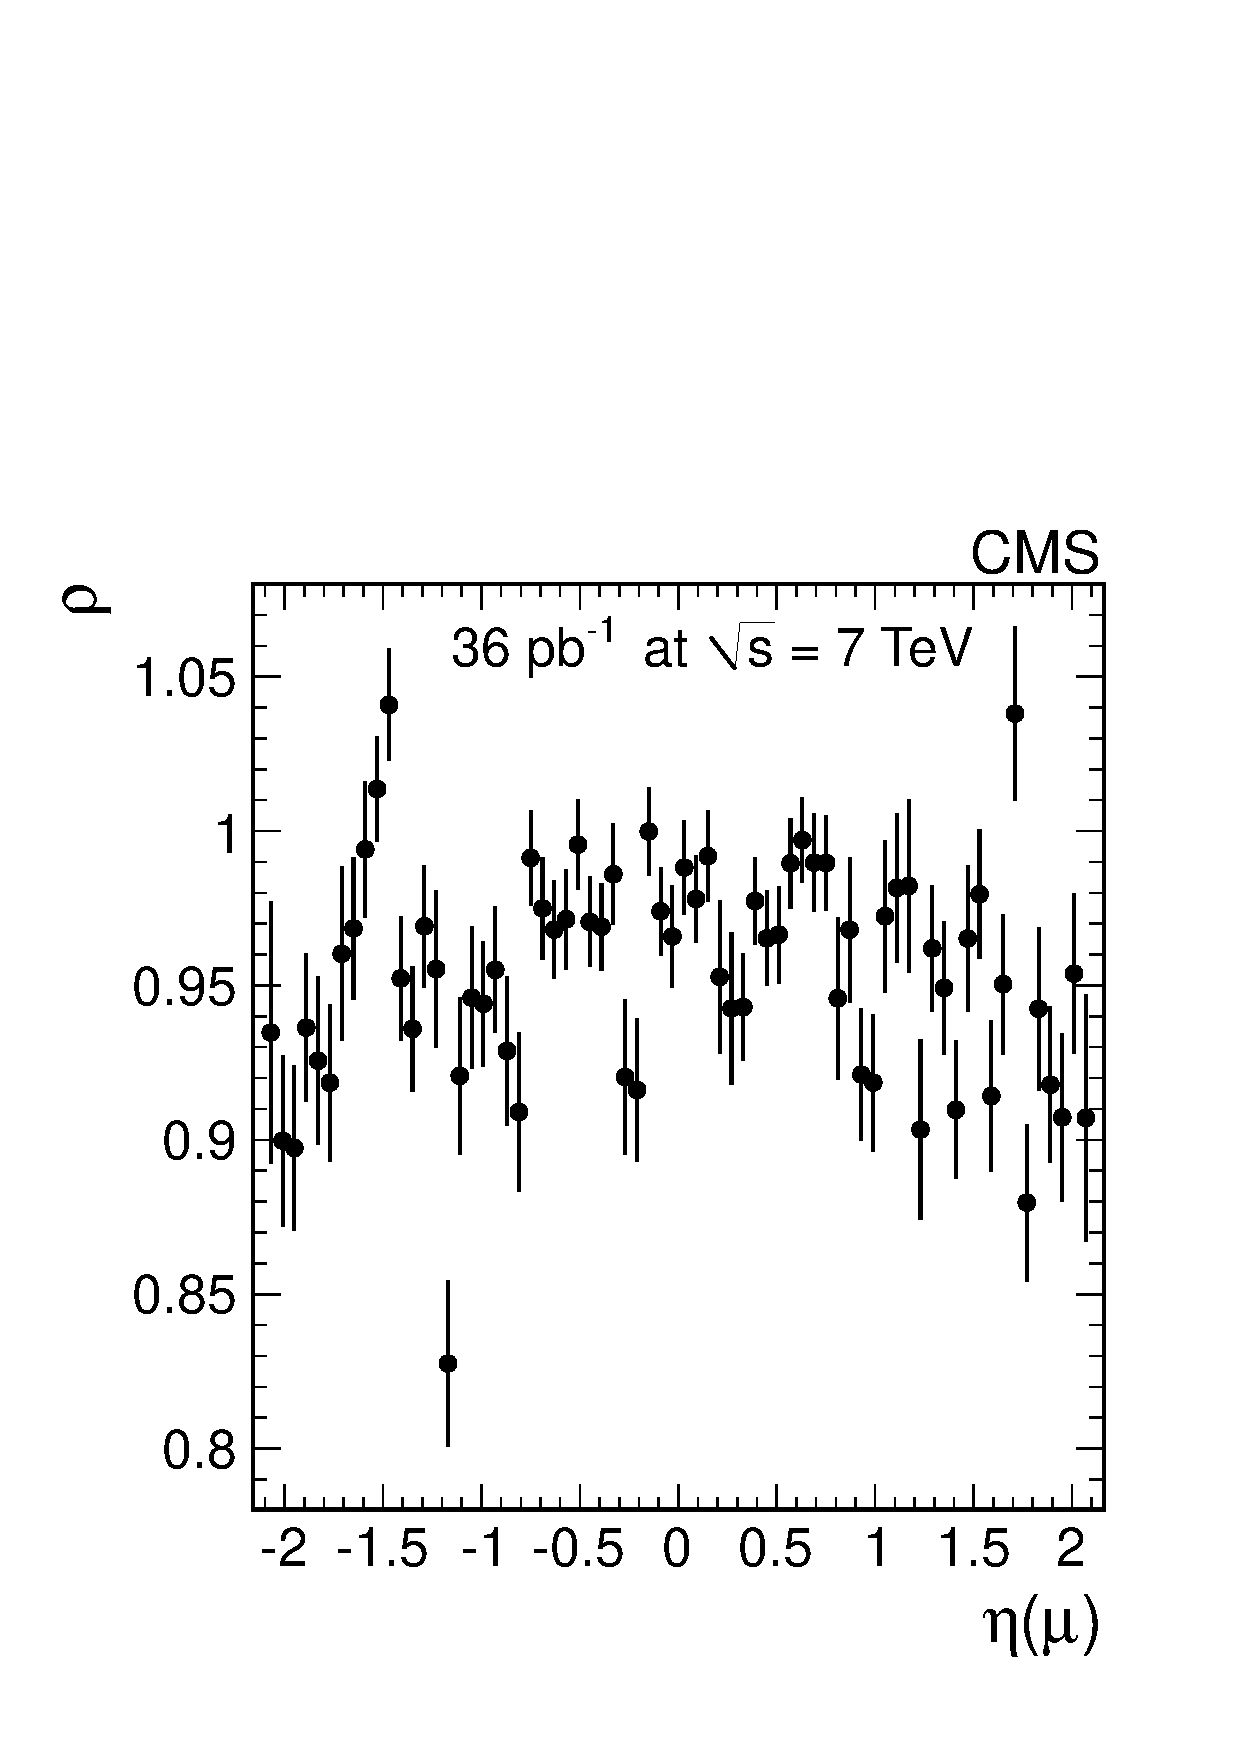
\includegraphics[width=7cm]{figs/correction_factor_eta.pdf}
%  \epsfig{figure=efficiency_eta.eps,width=0.50\linewidth}%
%  \epsfig{figure=correction_factor_eta.eps,width=0.5\linewidth}
  \end{center}
\caption{Single-muon efficiencies (left) for data (red circles with error bars)
 and simulation (black triangles), and the ratio between them (right), as a function of the muon $\eta$.}
\label{rho_eta}
\end{figure}
\begin{figure}
  \begin{center}
  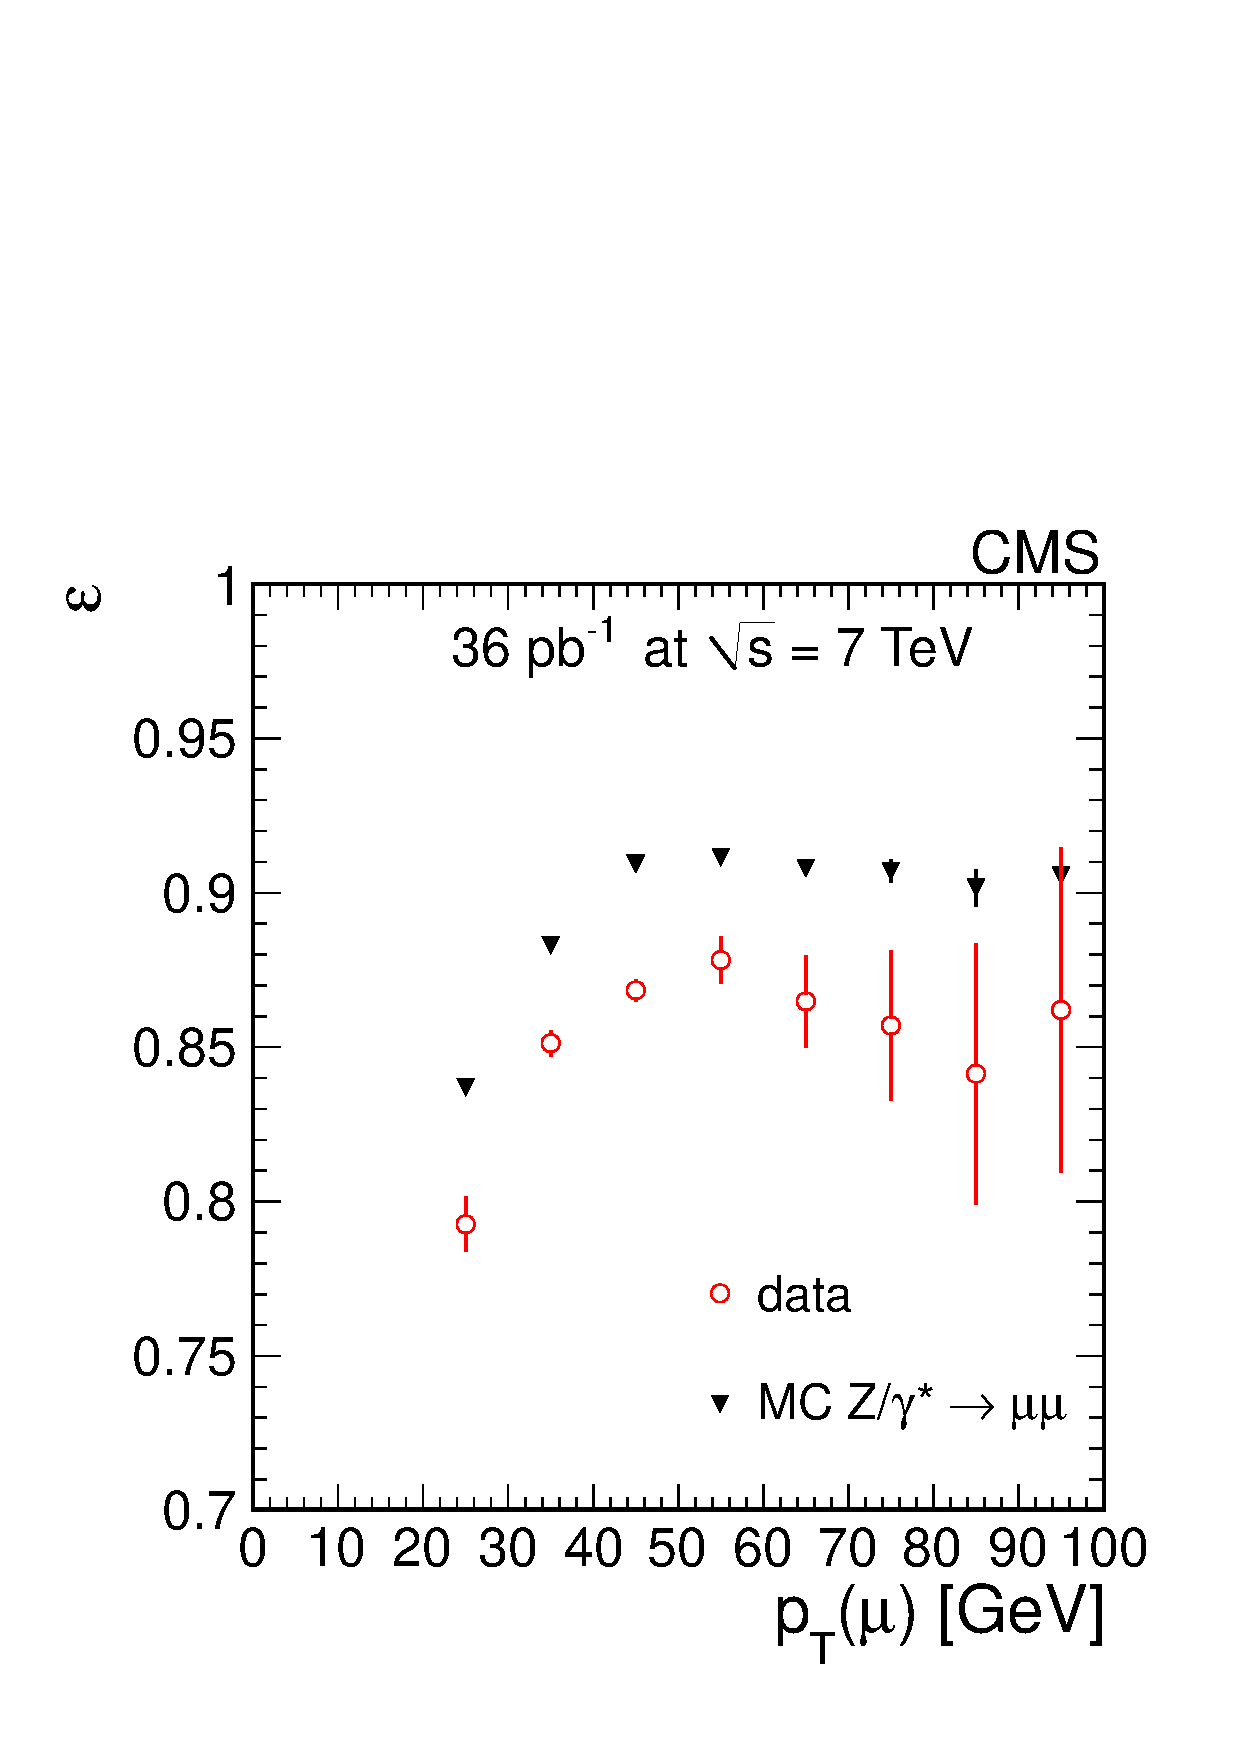
\includegraphics[width=7cm]{figs/efficiency_pt.pdf}%
  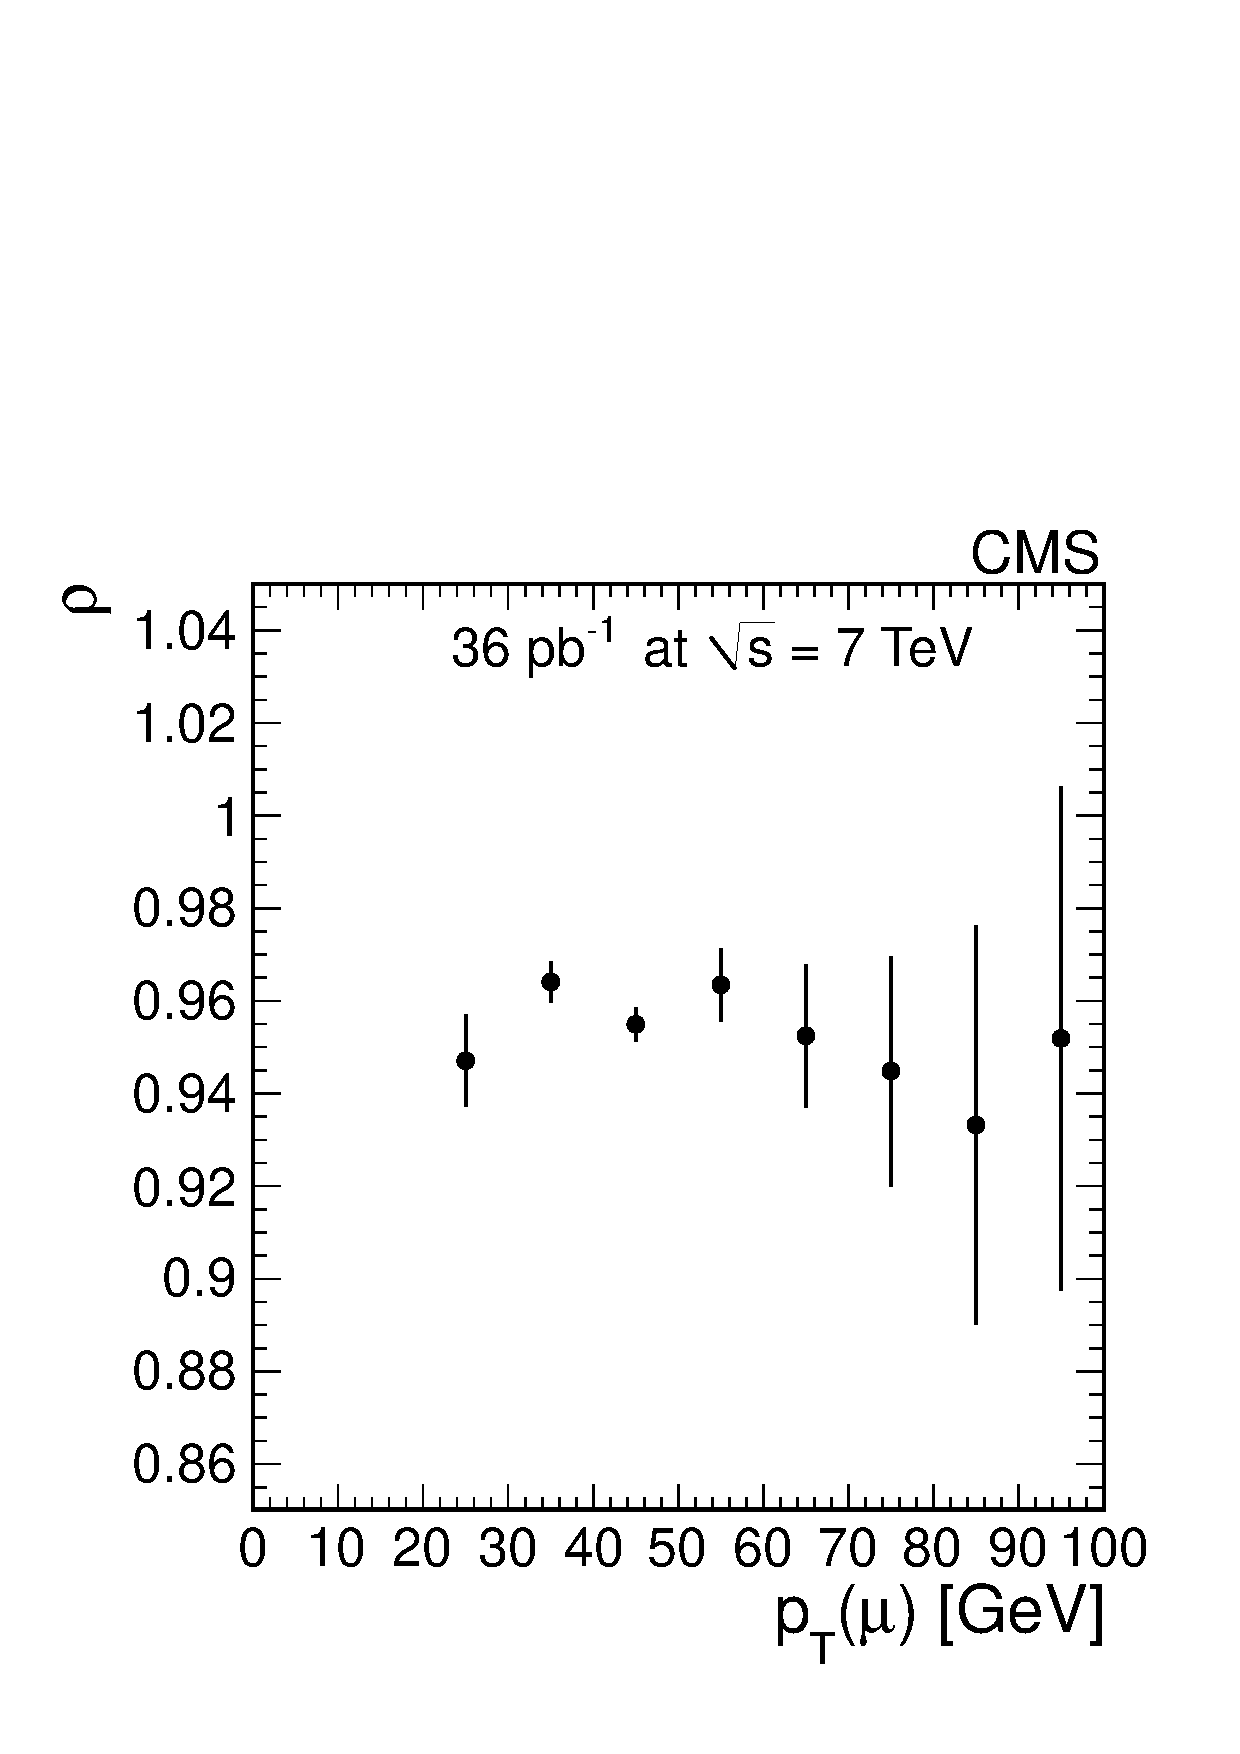
\includegraphics[width=7cm]{figs/correction_factor_pt.pdf}
%  \epsfig{figure=efficiency_eta.eps,width=0.50\linewidth}%
%  \epsfig{figure=correction_factor_eta.eps,width=0.5\linewidth}
  \end{center}
\caption{Single-muon efficiencies (left) for data (red circles with error bars)
and simulation (black triangles) and the ratio between them (right),
as a function of the muon $\Pt$.}
\label{rho_pt}
\end{figure}

The average single-muon efficiencies and correction factors are reported in Table~\ref{tab:effic_charge}
for positively and negatively charged muons separately, and inclusively.
The statistical uncertainties reflect the size of the available Z sample. Systematic uncertainties
on $\effTPdata$ and the correction factors $\rho$ are discussed in Section~\ref{sec:muonSyst}.

\begin{table}[htb] %
    \begin{center}
    \caption{Tag-and-probe efficiencies in data and simulation and correction factors
for positively and negatively charged muons.
The errors on  $\effTPmc$ are statistical only, while the systematic uncertainty is included for
the other quantities.
}
    \label{tab:effic_charge}
      \begin{tabular}{|l|c|c|c|} \hline
                    &            $\mu^+$            &            $\mu^-$           &                     $\mu^\pm$ \\ \hline\hline
        $\effTPdata$  & $(86.0 \pm 0.8)\%$ & $(85.0 \pm 0.8)\%$ & $(85.6 \pm 0.8)\%$ \\
        $\effTPmc$    & $(89.25 \pm 0.05 )\%$         & $(89.38 \pm 0.05)\%$         & $(89.32 \pm 0.04)\%$        \\
        $\rhoeff$   & $(96.3 \pm 0.9)\%$ & $(95.1 \pm 0.9)\%$& $(95.7 \pm 0.9)\%$\\
%         $\effTPdata$  & $(85.98 \pm 0.38 \pm 0.72)\%$ & $(85.00 \pm 0.36 \pm 0.72)\%$& $(85.48 \pm 0.27 \mathrm{(stat)} \pm  0.72 \mathrm{(syst)})\%$ \\
%         $\effTPmc$    & $(89.25 \pm 0.05 )\%$         & $(89.38 \pm 0.05)\%$         & $(89.32 \pm 0.04\, \mathrm{(stat)})\%$        \\
%         $\rhoeff$   & $(96.33 \pm 0.43 \pm 0.81)\%$ & $(95.09 \pm 0.40 \pm 0.81)\%$& $(95.70 \pm 0.30 \mathrm{(stat)} \pm  0.81\mathrm{(syst)})\%$\\

      \hline
      \end{tabular}
    \end{center}
  \end{table}

A small fraction of muon events are lost because of L1 muon trigger prefiring, i.e., the assignment
of a muon segment to an incorrect bunch crossing, occurring with a
probability of a few per mille per segment.
The effect is only sizable in the drift-tube system. The efficiency correction in the barrel region
is estimated for the current data to be ${\sim}1\%$ per muon. This estimate is
obtained from studies of muon pairs selected by online and offline single-muon trigger paths at
the wrong bunch crossing, that have an invariant mass near the Z mass.
Tracker information is not present in the case of prefiring, precluding the building of a
trigger muon online or a global muon in the offline reconstruction.
Since this effect is not accounted for in the efficiency from \TNP,
the measured $\Zmm$ and $\Wmn$ cross sections are increased by 1\% and 0.5\%,
respectively (including barrel and endcap regions)
to correct for the effect of trigger prefiring. The uncertainty on those corrections
is taken as a systematic uncertainty.

The $\Wmn$ efficiencies from simulation are shown in Table~\ref{tab:mu-MCeff} for the $\Wp$ and $\Wm$ samples separately
and combined after applying the binned corrections estimated with the \TNP method using Z events.


\begin{table}[ht] %
  \begin{center}
  \caption{Simulation efficiencies and final corrected efficiencies for the $\Wmn$ analysis.
The quoted uncertainties are statistical for $\effmc$ and include both statistical and systematic uncertainties
for the corrected efficiencies $\effmc \times \rhoeff$.
  \label{tab:mu-MCeff}}
  \begin{tabular}{|l|c|c|}
    \hline
   & $\effmc$ & $\effmc \times \rhoeff$ \\
    \hline\hline
 $\Wpmn$   & $(89.19\pm 0.03)\%$ & $(85.4\pm 0.8)\%$ \\
 $\Wmmn$   & $(89.19\pm 0.03)\%$ & $(84.1\pm 0.8)\%$ \\
 $\Wmn$  & $(89.19\pm 0.03)\%$ & $(84.8\pm 0.8)\%$ \\
    \hline
    \end{tabular}
  \end{center}
\end{table}



For the $\Zmm$ cross section measurement, the muon efficiencies are determined together with the Z yield using
a simultaneous fit described in Section~\ref{sec:Zmumu}, and efficiencies from a \TNP method were only applied to
a counting analysis used as cross check. The simulation efficiency obtained from the POWHEG Z samples, together
with the corrected Z selection efficiency $\effmc \times \rhoeff$ are shown in Table~\ref{tab:mu-Zeff}.

\begin{table}[ht] %
  \begin{center}
  \caption{ Simulation efficiency and the final corrected selection efficiency for the ~$\Zmm$ analysis.
The quoted uncertainties are statistical for $\effmc$ and include both statistical and
systematic uncertainties for the corrected efficiency $\effmc \times \rhoeff$.
 \label{tab:mu-Zeff}}
  \begin{tabular}{|l|c|c|}
    \hline
     & $\effmc$ & $\effmc \times \rhoeff$ \\
    \hline\hline
    $\Zmm$  & $(89.21\pm 0.05)\%$ & $(87.1\pm 1.1)\%$ \\
    \hline
    \end{tabular}
  \end{center}
\end{table} 